\section{Sentiment Analysis Model}
This section outlines the training, testing, and predicting of the BERT model, as well as the dataset chosen for fine-tuning and how it was pre-processed. Most of the functionality shown in this section is contained within the \pinline{BertModel} class under \pinline{toolkit/analysis/model.py}:

\begin{python}
class BertModel(object):
    """
    Class for sentiment analysis using BERT model.
    Attributes:
        tokeniser: BERT tokenizer for tokenizing input text.
        model: BERT model for sentiment classification.
    """
    def __init__(self) -> None:
        self.tokeniser, self.model = None, None
        self.load_model(toolkit.get_dir() + '/models/')
\end{python}

    \subsection{Training}
        This section will outline the steps taken to train and fine-tune the pre-trained BERT model. The majority of the functionality in this section takes place in the \pinline{train()} and \pinline{cross_validate()} methods.

        \subsubsection{Examining the Dataset}
        Before the model can be trained, an appropriate dataset for fine-tuning must be found. As this artefact focuses on social media sentiment analysis, a dataset that has pre-labelled social media posts based on sentiment is needed. For this use-case, the Sentiment140 dataset \citet{sentiment140dataset} was chosen as a widely used and praised dataset for fine-tuning BERT for social media sentiment analysis.

        When calling \pinline{describe()} on the dataset loaded as a Pandas \pinline{DataFrame}, the results are as shown in the table below. This shows that the dataset labels negative sentiment as `0', and positive sentiment as `4', and also appears to have an equal number of negative and positive entries. This quality will be useful as it prevents issues like model generalisation, class imbalance, and overfitting, while allowing for enhanced performance and better feature representation learning.

        \begin{table}[h]
            \centering
            \caption{Dataset description.}
            \label{tbl:datasetdescription}
            \begin{tabular}{c|c|c|c|c|c|c|c|c}
                & Count & Mean & Std & Min & 25\% & 50\% & 75\% & Max \\
                \hline\hline
                Target & 1.60e6 & 2.00 & 2.00 & 0.00 & 0.00 & 2.00 & 4.00 & 4.00 \\
            \end{tabular}
        \end{table}

        We can confirm this by plotting the dataset on a chart using \pinline{pyplot}:

        \begin{figure}[h]
            \centering
            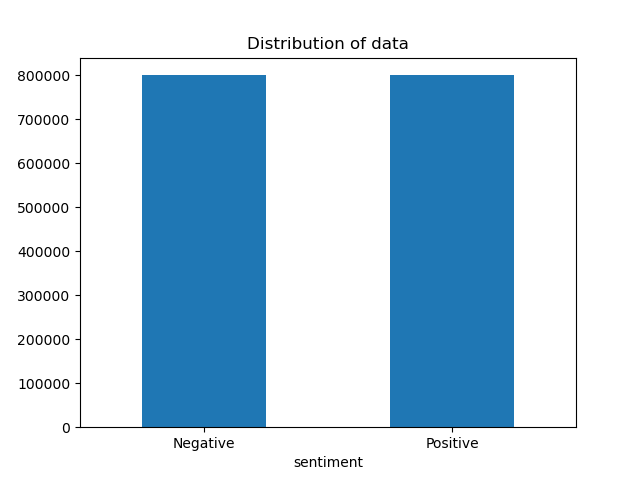
\includegraphics[width=0.6\textwidth]{figures/sentiment140-dataset-distribution.png}
            \caption{Classification distribution in the Sentiment140 dataset.}
        \end{figure}
        \FloatBarrier

        Further examination of the dataset can be accomplished by extracting a positively and negatively classified entry, the dataset provides six features for each post: Target (the sentiment polarity), ID, Date, Flag (the query), User, and Text (the body).

        \FloatBarrier
        \begin{table}[h]
            \centering
            \caption{Example of a positive post.}
            \label{tbl:positive_post}
            \begin{tabular}{p{0.15\linewidth} | p{0.6\linewidth}}
                Attribute & Value \\
                \hline\hline
                Target & 4 \\
                IDs & 1467822272 \\
                Date & Mon Apr 06 22:22:45 PDT 2009 \\
                Flag & NO\_QUERY \\
                User & ersle \\
                Text & I LOVE @Health4UandPets u guys r the best!! \\
            \end{tabular}
        \end{table}

        \begin{table}[h]
            \centering
            \caption{Example of a negative post.}
            \label{tbl:negative_post}
            \begin{tabular}{p{0.15\linewidth} | p{0.6\linewidth}}
                Attribute & Value \\
                \hline\hline
                Target & 0 \\
                IDs & 1467810369 \\
                Date & Mon Apr 06 22:19:45 PDT 2009 \\
                Flag & NO\_QUERY \\
                User & \_TheSpecialOne\_ \\
                Text & @switchfoot http://twitpic.com/2y1zl - Awww, that's a bummer.  You shoulda got David Carr of Third Day to do it. ;D \\
            \end{tabular}
        \end{table}
        \FloatBarrier

        \subsubsection{Pre-Processing the Data}
        Currently, the data is not fit for training purposes, to make it suitable the dataset must be cleaned up. Firstly, the dataset is loaded into a Pandas \pinline{DataFrame} using ISO-8859-1 encoding due to limitations with utf-8, then the unnecessary data can be removed from the dataset as it is loaded, as only the text and sentiment polarity are needed for training.

        \begin{python}
df = pd.read_csv(input_path, names=['sentiment', 'timestamp', 'datestring', 'N/A', 'user', 'text'], encoding='ISO-8859-1')
df = df[['text', 'sentiment']]
        \end{python}

        Next, the way sentiment is classified in the dataset must be changed; currently negative sentiment is labelled as `0' and positive is `4', this is changed to a simple binary classification where `0' is negative and `1' is positive.

        \begin{python}
df['sentiment'] = df['sentiment'].replace(4, 1)
        \end{python}

        The dataset should also be shuffled, this ensures that there are no related or similar tweets next to each other in the dataset.

        \begin{python}
toolkit.console("Shuffling dataset...")
df = df.sample(frac=1).reset_index(drop=True)
toolkit.console("Dataset shuffled.")
        \end{python}

        Now that the dataset has been prepared, the text of each post needs to be processed, for this purpose a class \pinline{TextProcessor} is defined to handle all processing.

        \begin{python}
class TextProcessor(object):
    def __init__(self):
        self.lemmatiser = WordNetLemmatizer()
        \end{python}
        
        The first function \pinline{preprocess()} is to remove various parts that will not contribute, or may even be detrimental, to the training of the model, such as urls, user mentions, etc. Firstly, several regex patterns are defined:

        \begin{python}
def preprocess(self, text: str) -> str:
    x_mention_pattern = r'@\S{4,}'
    ampersand_pattern = r'&amp;'
    url_pattern = r'((http://)[^ ]*|(https://)[^ ]*|( www\.)[^ ]*)'
    reddit_user_mention_pattern = r'/?u/\S+'
    reddit_sub_mention_pattern = r'/?r/\S+'
    newline_pattern = r'(\r\n|\r|\n)'
    reddit_url_match = r'/\[.*?(?=\]\((.*?)\))/g'
    reddit_url_replace = r'/\[.*?\]\(.*?\)/g'
        \end{python}

        Then \pinline{re.sub()} is called on the text for each substitution:

        \begin{python}
text = re.sub(x_mention_pattern, 'USER', text) # @user -> USER
text = re.sub(ampersand_pattern, '&', text) # &amp; -> &
text = re.sub(reddit_user_mention_pattern, 'USER', text) # /u/user or u/user -> USER
text = re.sub(reddit_sub_mention_pattern, 'SUBREDDIT', text) # /r/sub or r/sub -> SUBREDDIT
text = re.sub(url_pattern, 'URL', text) # https://link or http://link -> URL
text = re.sub(newline_pattern, ' ', text) # \\n -> ' '
        \end{python}

        Finally, for URLs on Reddit, which are in the format [shown text](URL hyperlink), all matches of Reddit's URL format are found, and replaced with just the text that would be shown to the user.

        \begin{python}
# Find all tags (text inside square brackets)
tags = [match.group(1) for match in re.finditer(r'\[(.*?)(?=\]\(.*?\))', text)]
# Replace all markdown links with the extracted tags
text = re.sub(r'\[.*?\]\(.*?\)', lambda match: tags.pop(0), text) # [name](link) -> name
        \end{python}

        There are also other optional functions that were experimented with for training in the \pinline{TextProcessor}: \pinline{lowercase()}, \pinline{lemmatise()}, and \pinline{soup()}, which toggle the text to lowercase, lemmatise and stem the text, and apply a \pinline{BeautifulSoup} html parser to the text, respectively.

        These functions are toggled off by default, but may be turned on by the user in settings. For further insight into these, visit the GitHub repository for the project \citep{sentimentanalysistool} (under \pinline{toolkit/data/preprocess.py}).

        \subsubsection{Training the Model}
        In the \pinline{BertModel}, a method \pinline{train()} for training the model is implemented, training on the Sentiment140 \citep{sentiment140dataset} dataset will fine-tune BERT to the specific linguistics and tone of social media. This function takes in a DataFrame containing the `text' and `sentiment' columns, along with the path to save the model to after training.

        \begin{python}
def train(self, dataset: pd.DataFrame, path: str) -> None:
        \end{python}

        Firstly, the data must be split into training, testing, and validation data. This is accomplished by leveraging Scikit-learn's \pinline{train_test_split()} method twice, initially for an 80/20 train/test split, then once more for a 80/10/10 split for separate testing and validation sets, ensuring robust evaluation metrics.

        \begin{python}
X_train, X_test, y_train, y_test = train_test_split(text, sentiment, test_size=1 - train_ratio, stratify=sentiment, random_state = 42)
X_val, X_test, y_val, y_test = train_test_split(X_test, y_test, test_size=test_ratio/(test_ratio + val_ratio), stratify=y_test, random_state=42)
        \end{python}

        After this, \pinline{self.model} and \pinline{self.tokeniser} are re-initialised to avoid interference from any previously stored configurations. Then the data is encoded using \pinline{self.tokenise()} to transform the text inputs into token IDs.

        \begin{python}
self.tokeniser = BertTokenizer.from_pretrained('bert-base-uncased', do_lower_case=True)
self.model = TFBertForSequenceClassification.from_pretrained('bert-base-uncased', num_labels=2)
        \end{python}

        Each value is encoded using \pinline{self.tokenise()} which takes a string `text' to transform the text inputs into token IDs.

        \begin{python}
self.tokeniser.batch_encode_plus(text, padding=True, truncation=True, max_length=128, return_tensors='tf') 
        \end{python}

        Following this, \pinline{self.fit_model()} is called, the model is compiled with an optimiser, loss function, and evaluation metrics. The Adam optimiser is used with a learning rate of 2e-5, and a sparse categorical cross-entropy loss function is defined to compute the difference between predicted and actual labels, with accuracy chosen as the evaluation metric for assessing model performance.

        \begin{python}
optimiser = tf.keras.optimizers.Adam(learning_rate=2e-5)
loss = tf.keras.losses.SparseCategoricalCrossentropy(from_logits=True)
metric = tf.keras.metrics.SparseCategoricalAccuracy('accuracy')
self.model.compile(optimizer=optimiser, loss=loss, metrics=[metric])
        \end{python}

        Finally, the model is fitted to the encoded data using \pinline{self.model.fit()}. This process trains the model on the training data while simultaneously validating its performance on the validation set. The batch size, which is the number of samples processed per gradient update, is set to 32, and the training process iterates over the dataset for 3 epochs.

        Through these iterations, the BERT model adapts its parameters to accurately classify the sentiment of the given social media post, enhancing its performance on this type of content.

        \begin{python}
history = self.model.fit([X_train_encoded['input_ids'], X_train_encoded['token_type_ids'], X_train_encoded['attention_mask']], np.array(y_train), validation_data=([X_val_encoded['input_ids'], X_val_encoded['token_type_ids'], X_val_encoded['attention_mask']], np.array(y_val)), batch_size=32, epochs=3)
        \end{python}

        \subsubsection{Cross-Validation}
        Cross-validation is a crucial element to evaluate the performance and robustness of a machine learning model. By splitting the dataset into multiple folds, cross-validation ensures that the model generalises well for unseen data, reducing the likelihood of overfitting, while also providing insight into the model's consistency across different subsets of data.

        This method is called at the end of the \pinline{train()} function instead of the single \pinline{self.fit_model()} call, if the user has enabled cross-validation. It takes in the training \pinline{DataFrame} and the number of splits \pinline{n_splits}, which defaults to 5. The text and sentiment columns of the dataset are converted into lists to be used later.

        \begin{python}
def cross_validate(self, dataset: pd.DataFrame, n_splits: int = 5) -> None:
    text = dataset['text'].tolist()
    sentiment = dataset['sentiment'].tolist()
        \end{python}

        Scikit-learn's \pinline{KFold} class is used to create cross-validation splits, shuffling the data before splitting to randomise the data.

        \begin{python}
kf = KFold(n_splits=n_splits, shuffle=True, random_state=42)
        \end{python}

        After initialising several empty lists for test loss, test accuracy, train accuracy, predicted labels, and actual labels, the function enters a loop which iterates through each fold; every iteration splits the data into training and validation sets, tokenises them, then fits and tests the model.

        \begin{python}
for train_index, val_index in kf.split(text):
    X_train, X_val = [text[i] for i in train_index], [text[i] for i in val_index]
    y_train, y_val = [sentiment[i] for i in train_index], [sentiment[i] for i in val_index]
    X_train_encoded = self.tokenise(X_train)
    X_val_encoded = self.tokenise(X_val)
    history = self.fit_model(X_train_encoded, y_train, X_val_encoded, y_val)
    test_loss, test_accuracy, pred_labels, actual_labels = self.test(X_val_encoded, y_val)
        \end{python}

        The results of each fold are appended to their corresponding, predefined lists for further analysis.

        \subsubsection{Testing the Model}
        In order to evaluate the model's performance on unseen data, it must be tested. This is done through the \pinline{test()} method, which takes the encoded test data in the form of a dictionary, and their corresponding labels in a list. The function returns key metrics such as test loss, test accuracy, and the predicted labels; these metrics help assess how well the model has generalised from the training data to the test data.

        \begin{python}
def test(self, X_test_encoded: dict, y_test: list[int]) -> tuple[float, float, list[str], list[str]]:
        \end{python}

        The model is evaluated on the test data using the \pinline{self.model.evaluate()} method.

        \begin{python}
test_loss, test_accuracy = self.model.evaluate([X_test_encoded['input_ids'], X_test_encoded['token_type_ids'], X_test_encoded['attention_mask']], np.array(y_test))
        \end{python}

        Then predictions are made using the \pinline{self.model.predict()} method, which returns logits. Using TensorFlow's \pinline{argmax()} function, the predicted labels can be obtained, which are then converted to a NumPy array and then their sentiment as a string using list comprehensions.

        \begin{python}
pred = self.model.predict([X_test_encoded['input_ids'], X_test_encoded['token_type_ids'], X_test_encoded['attention_mask']])
logits = pred.logits
pred_labels = tf.argmax(logits, axis=1)
pred_labels = pred_labels.numpy()
labels = {1: 'Positive', 0: 'Negative'}
pred_labels = [labels[i] for i in pred_labels]
actual_labels = [labels[i] for i in y_test]
        \end{python}

    \subsection{Predictions}
    The \pinline{predict()} function is designed to leverage the batch-processing and parallel-processing capabilities of BERT and TensorFlow, allowing for efficient sentiment prediction with a list of inputs of any length. It takes a list of strings to analyse, and returns the predicted sentiment labels for each input string.

    \begin{python}
def predict(self, text: list[str]) -> list[str]:
    \end{python}

    Initially, the input text is tokenised using the \pinline{self.tokenise()} method, which encodes the text into input IDs, token type IDs, and attention masks. These encoded values are then passed to the \pinline{self.model.predict()} function to get the predictions.

    \begin{python}
input_ids, token_type_ids, attention_mask = self.tokenise(text).values()
prediction = self.model.predict([np.array(input_ids), np.array(token_type_ids), np.array(attention_mask)])
    \end{python}

    Next, the prediction logits are processed to obtain the probability distributions over the classes using TensorFlow's \pinline{softmax()} function, and the confidence for each prediction is determined by the maximum probability value.

    \begin{python}
pred_logits = prediction.logits
pred_probs = tf.nn.softmax(pred_logits, axis=1).numpy()
pred_confidence = np.max(pred_probs, axis=1)
    \end{python}

    Finally, the predicted labels are determined using TensorFlow's \pinline{argmax()} function on the logits. The labels are mapped to their corresponding sentiment labels `Positive' or `Negative'. However, if the confidence score of a prediction is less than the threshold defined by the user, it is labelled as `Neutral'.

    \begin{python}
labels = {1: 'Positive', 0: 'Negative'}
pred_label_indices = np.argmax(pred_logits, axis=1)
pred_labels = [labels[i] if confidence >= confidence_threshold else 'Neutral' for i, confidence in zip(pred_label_indices, pred_confidence)]
    \end{python}

    The function then returns the predicted labels for further analysis.

\section{Social Media Data Collection}
The following section details the methods used to collect data from social media platforms for sentiment analysis. The data collection functionality is implemented within the \pinline{XScraper} and \pinline{RedditScraper} classes in \pinline{toolkit/data/social.py}. Unfortunately, due to new limitations with the free version of the X API which prevent searching posts, the \pinline{XScraper} class is not fully implemented and will be excluded from this section.

The \pinline{RedditScraper} class is used to scrape post data from Reddit, including comments if the user's configuration calls for it, using the PRAW library

\section{Database Management}

\section{Data Visualisation}

\section{Graphical User Interface}

\section{Other Implementations}